\documentclass{beamer}
% \usetheme{Berkeley}
% \usetheme{Madrid}
\usetheme{Warsaw}

\usepackage{xcolor}
\usepackage{xeCJK}
\setCJKmainfont{WenQuanYi Micro Hei Mono}


\title{机器学习基本原理与实践}
\author{王超}
\institute{}
\date{\today}


\begin{document}

% Frame 0
\frame{\titlepage}
% \frame{\tableofcontents}


% Frame 1
\begin{frame} {机器学习的两大基本问题} 

\begin{block}{分类问题(Classification)}
    {
    程序输出: N维向量(对应N种可能的分类对象的概率, 例如[Dog: 0.75, Cat: 0.20, Duck: 0.05])
    \begin{figure}
    \begin{center}
    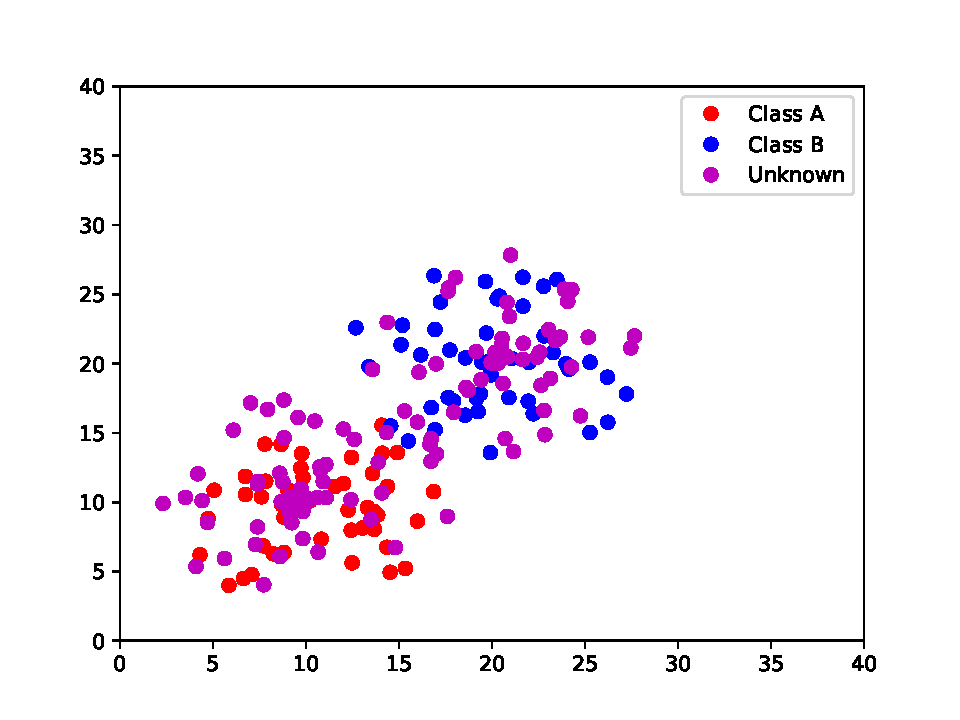
\includegraphics[width=0.6\textwidth]{fig/classification.pdf}
    \caption{分类问题}
    \end{center}
    \end{figure}
    }
\end{block}

\end{frame}



% Frame 2
\begin{frame} {机器学习的两大基本问题} 

\begin{block}{回归问题(Regression), 即求值}
    {
    程序输出: 标量

    }
\end{block}

\end{frame}

\end{document}